\section{Quantization and obstruction}\label{sec:qo}
In the \nameref{sec:bv}, we want to find an $\infty$-dimensional $(-1)$-symplectic geometry $(\cE,Q,\omega)$ to describe the QFT.
We have the classical data: the space of \textbf{local functionals}, $\cO_{\text{loc}}(\cE)\subset \cO(\cE)$, in which the classical interaction $I_0=\int_X \cL$ is an element of $\cO_{\text{loc}}(\cE)$. $I_0$ solves the CME: $QI_0+\hf \lcb I_0,I_0\rcb_0=0$. Here $\lcb -,-\rcb_0$ is the BV bracket with respect to the BV kernel $K_0=\omega^{-1}$ and is well-defined on $\cO_{\text{loc}}(\cE)$. However the BV operator $\Delta_0$ is ill-defined on $\cO_{\text{loc}}(\cE)$ and $\cO(\cE)$, where the naive QME $QI_0+\hbar \Delta_0 I_0+\hf \lcb I_0,I_0\rcb=0$ does not make sense.

One way out of this problem is to use regularization to define an effective QME. We defined the Poisson kernel $K_0=K_r+QP_r$, leading to a well-defined BV operator $\Delta_r$ on $\cO(\cE)$. For each $r$, we construct $I[r]\in \cO(\cE)$ solving the effective QME:
\bea \lb Q+\hbar\Delta_r\rb e^{I[r]/\hbar}=0\eea
and different regularizations are related by the homotopy RG (HRG) flow:
\bea e^{I[r']/\hbar}=\exp{\lb \hbar \p_{P^{r'}_r}\rb} e^{I[r]/\hbar}.\eea
We have seen that the effective QME and the HRG are compatible.
\bea
\tikzset{every picture/.style={line width=0.75pt}} %set default line width to 0.75pt    
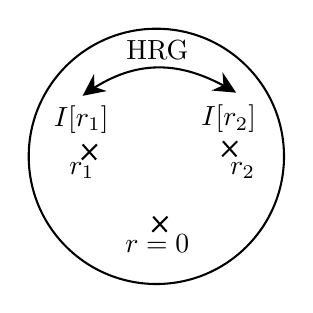
\begin{tikzpicture}[x=0.75pt,y=0.75pt,yscale=-1,xscale=1]
%uncomment if require: \path (0,300); %set diagram left start at 0, and has height of 300

%Shape: Circle [id:dp6926154379932559] 
\draw   (50,84.5) .. controls (50,50.53) and (77.53,23) .. (111.5,23) .. controls (145.47,23) and (173,50.53) .. (173,84.5) .. controls (173,118.47) and (145.47,146) .. (111.5,146) .. controls (77.53,146) and (50,118.47) .. (50,84.5) -- cycle ;
%Straight Lines [id:da2262569241568375] 
\draw    (75.98,78.77) -- (82.47,86.03) ;
%Straight Lines [id:da9042410789635242] 
\draw    (75.59,86.03) -- (82.85,78.77) ;

%Straight Lines [id:da7965197666945929] 
\draw    (143.59,77.24) -- (150.08,84.5) ;
%Straight Lines [id:da23412451653488264] 
\draw    (143.2,84.5) -- (150.46,77.24) ;

%Straight Lines [id:da694164688117211] 
\draw    (109.97,113.53) -- (116.47,120.79) ;
%Straight Lines [id:da27199650302361067] 
\draw    (109.59,120.79) -- (116.85,113.53) ;

%Curve Lines [id:da21026083909699889] 
\draw    (78.71,53.37) .. controls (106.69,33.96) and (129.65,42.23) .. (147.47,52.37) ;
\draw [shift={(149.95,53.81)}, rotate = 210.62] [fill={rgb, 255:red, 0; green, 0; blue, 0 }  ][line width=0.08]  [draw opacity=0] (10.72,-5.15) -- (0,0) -- (10.72,5.15) -- (7.12,0) -- cycle    ;
\draw [shift={(75.98,55.34)}, rotate = 323.13] [fill={rgb, 255:red, 0; green, 0; blue, 0 }  ][line width=0.08]  [draw opacity=0] (10.72,-5.15) -- (0,0) -- (10.72,5.15) -- (7.12,0) -- cycle    ;

% Text Node
\draw (68.07,86.16) node [anchor=north west][inner sep=0.75pt]    {$r_{1}$};
% Text Node
\draw (145.59,86.16) node [anchor=north west][inner sep=0.75pt]    {$r_{2}$};
% Text Node
\draw (95.02,120.54) node [anchor=north west][inner sep=0.75pt]    {$r=0$};
% Text Node
\draw (60.62,58.71) node [anchor=north west][inner sep=0.75pt]    {$I[r_{1}]$};
% Text Node
\draw (131.67,58.33) node [anchor=north west][inner sep=0.75pt]    {$I[r_{2}]$};
% Text Node
\draw (95.53,27.36) node [anchor=north west][inner sep=0.75pt]   [align=left] {HRG};
\end{tikzpicture}
\eea


\subsection*{Heat kernel regularization}
Typically, fixing a choice of metric, we have 
\begin{itemize}
    \item the adjoint of $Q:\cE\to \cE$, denoted as $Q^\dagger: \cE\to \cE$,
    \item a generalized Laplacian, $\lsb Q,Q^\dagger\rsb= QQ^\dagger+Q^\dagger Q$ 
\end{itemize}
Hence we can define a heat operator $e^{-L\lsb Q,Q^\dagger\rsb}$ for $L>0$. Let $K_L\in \sym^2(\cE)$ be the kernel of the heat operator by 
\bea \lb e^{-L\lsb Q,Q^\dagger\rsb}\alpha\rb \lb x\rb
=\int dy \lan K_L(x,y),\alpha(y)\ran\quad \text{for }\alpha\in\cE.\eea 
Here $\lan-,-\ran$ is the pairing from $\omega$. Note that
\begin{itemize}
    \item $K_0=\lim_{L\to 0} K_L$ is the $\delta$-function distribution $\omega^{-1}$,
    \item $K_L\in \sym^2(\cE)$ is smooth for $L>0$.
\end{itemize}

Let $P_L$ be the kernel of the operator $\int_0^L dt\ Q^\dagger e^{-t\lsb Q,Q^\dagger\rsb} $. Explicitly, we have 
\bea P_L= \int_0^L dt \lb Q^\dagger \otimes 1\rb K_t.\eea
The operator equation 
\bea \lsb Q, \int_0^L dt\ Q^\dagger e^{-t\lsb Q,Q^\dagger\rsb} \rsb 
= \int_0^L dt \lsb Q,Q^\dagger\rsb e^{-t\lsb Q,Q^\dagger\rsb} 
=1=e^{-L\lsb Q,Q^\dagger\rsb}.\eea
This is translated into the kernel equation:
\bea K_0-K_L=(Q\otimes 1+1\otimes Q)P_L\eea
or simply written as
\bea K_0-K_L=QP_L.\eea

We can use $K_L$ to define the effective QME. For $0<\vep<L$, similarly the operator equation is 
\bea \lsb Q, \int_\vep^L dt\ Q^\dagger e^{-t\lsb Q,Q^\dagger\rsb} \rsb 
=e^{-\vep\lsb Q,Q^\dagger\rsb}-e^{-L\lsb Q,Q^\dagger\rsb}\eea
or 
\bea K_\vep-K_L=(Q\otimes 1+1\otimes Q)P_\vep^L,\eea
where $P^L_\vep= \int_\vep^L dt \lb Q^\dagger \otimes 1\rb K_t$ is called the {\em regularized propagator}. Now we can use $P^L_\vep$ to connect the effective QME at $\vep$ with the effective QME at $L$ via the homotopy RG, $\exp{\lb \hbar\p_{P_\vep^L}\rb}$.

\subsection*{Constructing effective BV quantization using heat kernel regularization}
\paragraph{Step 1: The method of counter-term.}
Let $I_0\in \cO_{\text{loc}}(\cE)$ be the classical interaction. Since $P_0^L$ is singular, the limit $\lim_{\vep\to 0} \exp{\lb \hbar\p_{P_\vep^L}\rb} e^{I_0/\hbar}$ does not exist. Pictorially, all the loop diagrams, such as
\bea 
    \begin{fmffile}{fddlim}
    \begin{tabular}{c}
        \begin{fmfgraph*}(100,50)
                \fmfleft{i1,i2}
                \fmfright{o1,o2}
                \fmf{plain,tension=4}{i1,v1}
                \fmf{plain,tension=4}{i2,v1}
                \fmf{plain,tension=4}{v2,o1}
                \fmf{plain,tension=4}{v2,o2}
                \fmf{plain,left,label=$P_\vep^L$,label.side=left,tension=3}{v1,v2,v1}
                \fmfv{label=$I_0$,label.angle=170,decor.shape=circle,decor.filled=full,decor.size=2thick}{v1}
                \fmfv{label=$I_0$,label.angle=10,decor.shape=circle,decor.filled=full,decor.size=2thick}{v2}
        \end{fmfgraph*}
        \end{tabular}
    \end{fmffile}
\eea
are divergent as $\vep\to 0$.

We can find a {\em counter-term} $I^\eps\in \hbar \cO_{\text{loc}}(\cE)\llb \hbar\rrb$ which is $\vep$-dependent and is singular as $\vep\to 0$ such that
\bea \lim_{\vep\to 0} \exp{\lb \hbar\p_{P_\vep^L}\rb} e^{\lb I_0+I^\eps\rb/\hbar}\coloneqq e^{I[L]^{\text{naive}}/\hbar}\eea exists. 
Such defined $I[L]^{\text{naive}}$ has the following advantage for $0<L_1<L_2$, 
\bea e^{I[L_2]^{\text{naive}}/\hbar}
&= \lim_{\vep\to 0} \exp{\lb \hbar\p_{P_\vep^{L_2}}\rb} e^{\lb I_0+I^\eps\rb/\hbar}\\
&= \lim_{\vep\to 0} \exp{\lb \hbar\p_{P_{L_1}^{L_2}}\rb} \exp{\lb \hbar\p_{P_\vep^{L_1}}\rb} e^{\lb I_0+I^\eps\rb/\hbar} \quad \text{using } P_\vep^{L_2}=P_{L_1}^{L_2}+P_\vep^{L_1}\\
&= \exp{\lb \hbar\p_{P_{L_1}^{L_2}}\rb} \lim_{\vep\to 0} \exp{\lb \hbar\p_{P_\vep^{L_1}}\rb} e^{\lb I_0+I^\eps\rb/\hbar} \quad \text{since } P_{L_1}^{L_2} \text{ is smooth}\\
&= \exp{\lb \hbar\p_{P_{L_1}^{L_2}}\rb} e^{I[L_1]^{\text{naive}}/\hbar}.
\eea
In other words, the family $\lcb I[L_1]^{\text{naive}}\rcb_{L>0}$ satisfies the homotopy RG. However, $\lcb I[L_1]^{\text{naive}}\rcb_{L>0}$ may not satisfy the QME.

\paragraph{Step 2: Further corrections.}
Adjust $I^\eps$ to $\Tilde{I}^\eps$ by finding further corrections such that
\bea e^{I[L]/\hbar}
&= \lim_{\vep\to 0} \exp{\lb \hbar\p_{P_\vep^{L}}\rb} e^{\lb I_0+\Tilde{I}^\eps\rb/\hbar}.\eea
Then the defined limit $I[L]$ satisfies the QME.

\begin{rmk}
Step 1 is always possible.
Step 2 is NOT always possible; it might have {\em obstructions}, in physics this is called the {\em gauge anomaly}.
\end{rmk}

\begin{rmk}
There are cases where $\vep$-dependent counter-terms are not required in the sense that the limit 
\bea e^{I[L]/\hbar}
&= \lim_{\vep\to 0} \exp{\lb \hbar\p_{P_\vep^{L}}\rb} e^{I/\hbar}\eea
exists for a large class of local $I\in \cO_{\text{loc}}(\cE)\llb\hbar\rrb$. Such a theory is called \textbf{ultraviolet (UV)-finite}. Then we can explore the meaning of the effective QME $\lb Q=\hbar \Delta_L\rb e^{I[L]/\hbar}=0$ or $QI[L]+\hbar \Delta_L I[L]+\hf \lcb I[L],I[L]\rcb_L=0$. The upshot is that $L\to 0$ has a meaning in which the effective QME is reduced to $QI+\hf \lsb I,I\rsb=0$, where $\lsb-,-\rsb$ is the {\em quantum deformed bracket}.
\end{rmk}

We will explain two main UV-finite examples:
\bi[(1)]
\item Chern-Simons type topological theory.
\item In particular, we will discuss topological quantum mechanics (2d chiral theory).
\ei

\subsection*{Deformation-Obstruction theory}
Let's first consider the quantization problem CME $\leadsto$ QME in a DGBV $\lb \cA,Q,\Delta\rb$. Let $I_0\in \cA_0$ solve the CME $QI_0+\hf \lcb I_0,I_0\rcb=0$. Our goal is to find 
\bea I=I_0+I_1\hbar+I_2\hbar^2+\cdots \in \cA\llb \hbar\rrb\eea
solving the QME $QI+\hbar\Delta I+\hf \lcb I,I \rcb=0$.

\paragraph{Strategy:} find $I_1,I_2,\cdots$ in order of $\hbar$.
\bea QI+\hbar\Delta I+\hf \lcb I,I \rcb=\cO(\hbar^{n+1})\quad (n\geq 0).\eea 
\begin{itemize}
    \item $n=0$: this is the initial data of CME $QI_0+\hf \lcb I_0,I_0\rcb=0$.
    \item $n=1$: $\hbar$-term gives $QI_1+\Delta I_0+\lcb I_0,I_1 \rcb=0$. We need to find $I_1$ solving the above equation. Let us write it as 
    \bea QI_1+\lcb I_0,I_1 \rcb=\Delta I_0. \eea
    For convenience, let us denote $\delta=Q+\lcb I_0,-\rcb$. The CME implies that $\delta^2=0$. We need to solve 
    \bea \delta I_1=-\Delta I_0.\eea
    A key observation is that $\delta\lb -\Delta I_0\rb=0$ (exercise). So we see that $-\Delta I_0$ is $\delta$-closed. The solvability of $I_1$ asks whether $-\Delta I_0$ is $\delta$-exact. Let $\cO_1=\Delta I_0$ and let $\lsb \cO_1\rsb\in H^1(\cA,\delta)$ be the corresponding $\delta$-cohomology class. Then
    \begin{prop}
    $I_1$ can be solved $\LRA \lsb \cO_1\rsb=0$ in $H^1(\cA,\delta)$.
    \end{prop}
    Assume $\lsb \cO_1\rsb=0$. Let $I_1$ and $\Tilde{I}_1$ be two solutions. Then
    \bea \delta(I_1-\Tilde{I}_1)=0 \RA \Tilde{I}_1-I_1 \text{ is } \delta-\text{closed}.\eea
    Also, for any $J\in \cA_0$, the solution
    \bea I_1+\delta J \sim I_1,\eea
    where $\sim$ denotes that both sides are gauge equivalent in a suitable sense (i.e. solving a family version of QME along an interval).
    \begin{prop}
    If $I_1$ can be solved, then
    \bea \lcb \text{solution of } I_1\rcb/ \text{gauge}= H^0(\cA,\delta).\eea
    \end{prop}
    
    \item $n>1$: Assume we have found 
    \bea I_{<k}\coloneqq I_0+I_1\hbar +\cdots+I_{k-1} \hbar^{k-1}\eea
    solving $QI_{<k}+\hbar\Delta I_{<k}+\hf \lcb I_{<k},I_{<k}\rcb=\cO(\hbar^k)$. Let's consider the problem of solving $I_k$. The above equation can be written as 
    \bea \lb Q+\hbar\Delta\rb e^{I_{<k}/\hbar}=\cO(\hbar^{k-1})e^{I_{<k}/\hbar}.\eea
    We want to find $I_k$ such that 
    \bea \lb Q+\hbar\Delta\rb e^{\lb I_{<k}+I_k\hbar^k\rb/\hbar}=\cO(\hbar^{k})e^{\lb I_{<k}+I_k\hbar^k\rb/\hbar}.\eea
    Let us write
    \bea \lb Q+\hbar\Delta\rb e^{I_{<k}/\hbar}=\lb \cO_k\hbar^{k-1}+\cO(\hbar^k)\rb e^{I_{<k}/\hbar},\eea
    where $\cO_k$ is the leading term in $\cO(\hbar^{k-1})$.
    Explicitly, we have
    \bea QI_{<k}+\hbar \delta I_{<k}+\hf \lcb I_{<k},I_{<k}\rcb=\cO_k \hbar^k+\cO(\hbar^{k+1}).\eea
    Similarly, we need to solve
    \bea Q\lb I_{<k}+\hbar^k I_{k}\rb+\hbar\lb \Delta I_{<k}+\hbar^k I_{k}\rb+\hf \lcb I_{<k}+\hbar^k I_{k}, I_{<k}+\hbar^k I_{k}\rcb= \cO(\hbar^{k+1}).\eea
    This is equivalent to $QI_{k}+\lcb I_{0},I_{k}\rcb=\cO_k$ or $\delta I_{k}=\cO_k$.
    \begin{clm}
    $\cO_k$ is $\delta$-closed.
    \end{clm}
    \begin{sproof}
    Since $(Q+\hbar\Delta)$ to both sides of
    \bea \lb Q+\hbar\Delta\rb e^{I_{<k}/\hbar}=
    \lb \cO_k \hbar^{k-1}+\cO(\hbar^k)\rb e^{I_{<k}/\hbar}\eea
    and use the fact that $\lb Q+\hbar\Delta\rb^2=0$. Then $Q\cO_k+\lcb I_0,\cO_k\rcb=0$. The solvability of $I_k$ asks whether $\cO_k$ is $\delta$-exact.
    \end{sproof}
    \begin{prop}
    Solvability of $I_k \LRA \lsb \cO_k\rsb=0$ in $H^1(\cA,\delta)$. Moreover, if $I_k$ can be solved, then 
    \bea \lcb \text{solution of } I_k\rcb/ \text{gauge}= H^0(\cA,\delta).\eea
    \end{prop}
    \begin{rmk}
    \begin{itemize}
        \item $\lsb\cO_k\rsb\in H^1(\cA,\delta)$ is the \textbf{obstruction class} (\textbf{gauge anomaly}) for solving QME up to $\hbar^k$,
        \item $H^1(\cA,\delta)$ is the \textbf{obstruction space},
        \item $H^0(\cA,\delta)$ is the \textbf{tangent space} (or \textbf{deformation space}).
    \end{itemize}
    \end{rmk}
    In particular, we have proved
    \begin{thm}
    If $H^1\lb\cA, Q+\lcb I_0,-\rcb\rb=0$, then there exists a quantization $I=I_0+\hbar I_1+\cdots$ solving the QME $QI+\hbar\Delta I+\hf \lcb I,I\rcb=0$.
    \end{thm}
\end{itemize}

\subsection*{Effective QME}
In the QFT case, things are more complicated since we need to deal with regularization. However, the good thing is that the analogue of deformation-obstruction theory still exists. The relevant complex is $\lb \cO_{\text{loc}}\lb \cE\rb, Q+\lcb I_0,-\rcb\rb$. Note that $Q+\lcb I_0,-\rcb$ is well-defined on local functionals and CME implies that $\lb \cO_{\text{loc}}\lb \cE\rb, Q+\lcb I_0,-\rcb\rb$ indeed forms a complex.

Similar to the above discussion, we have 
\begin{thm}\label{thm5.2}
The obstruction space for effective BV quantization of $I_0$ is given by
\bea H^1\lb \cO_{\text{loc}}\lb \cE\rb, Q+\lcb I_0,-\rcb\rb.\eea
The tangent space (deformation space) is
\bea H^0\lb \cO_{\text{loc}}\lb \cE\rb, Q+\lcb I_0,-\rcb\rb.\eea
\end{thm}

\begin{rmk}
The locality is important and allows the computation of the above cohomologies via $D$-module methods.
\end{rmk}

\noindent \textsc{Reference}:
Theorem \ref{thm5.2} has many different setups and versions in the literature. The discussion we follow here is 
\cite{costello2011renormalization}, which also contains the references for classical works.






